\section{Adaptive measurement theory}\label{sec:th}
\subsection{Conception}
The majority of experiments obey the following principal scheme: the ``black box'' (our system) produces some output and we try to find parameters of this system using just this signal (see Fig.\ref{pic:stfilt}). There are two contributions to it: dynamic processes in our system and noises acting on it. 
All the information about values we want to know contains in the signal part of the output and noises only disturb us - obviously, we wish to get rid
of the them. This task can be solved by means of filtering theory: we estimate desired parameters from noisy signal, applying so-called filtering 
operator to the output. The choice of this estimation procedure depends on the particular problem, but the conception stays mostly the same - we choose
it to satisfy some criteria, such as minimal mean square error.

Adaptive measurements in general and adaptive filtering in particular involve using this filtering approach\cite{Wiseman2011a,Ahn2008}. The simple adaptive procedure is:
measurement - estimation the parameters - adjust measurement device - new measurement. Many researches apply this idea in classical experiments, but 
is quantum physics there are only few research groups working on this task\cite{Wiseman1997,Braginsky1993}. Wiseman and colleagues in made significant contribution to the adaptive filtering and
control theory \cite{Berry2008,Berry2001,Berry2002,Measurements1995m}. By the moment there are a few works on adaptive research in GW detectors \cite{Hentschel2010,Dhurandhar2008}.

\subsection{System}

\begin{figure}
\center{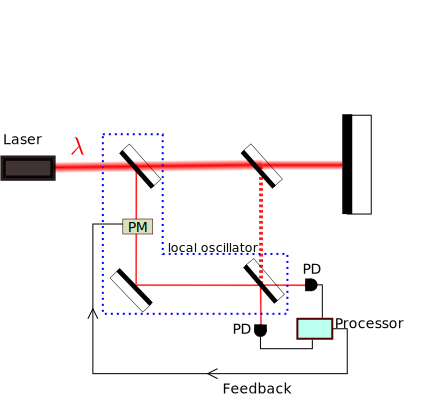
\includegraphics[width=0.5\textwidth]{adaptive_scheme}}
\caption{Optomechanical system}
\label{scheme}
\end{figure}

We consider simple optomechanical system of oscillator and homodyne detector (see Fig.\ref{scheme})\\
The oscillator can be described with following equation of motion:
\begin{equation}
\begin{cases}
 \dot{\hat{x}}(t) &= \frac{\hat{p}(t)}{m},\\
 \dot{\hat{p}}(t) &= -2\gamma \hat{p}(t) - m\omega_m^2 \hat{x}(t) + \alpha \hat{a}_1(t),
\end{cases}
\end{equation}
where $\alpha \hat{a}_1(t)$ corresponds to back-action noise, $\alpha$ is coupling constant between the oscillator and optical field.
So, for the ingoing optical fields $\hat{a}_{1,2}$ and outgoing $\hat{b}_{1,2}$ (see Fig. \ref{pic:sys}) we get following input-output relations:
\begin{equation}
\begin{cases}
 \hat{b}_1(t) &= \hat{a}_1(t),\\
 \hat{b}_2(t) &= \hat{a}_2(t) + \frac{\alpha}{\hbar}\hat{x}(t)\label{b2_general}.
\end{cases}
\end{equation}

Here we introduced ingoing and outgoing optical fields. In the paraxial and narrowband approximation they are related with strength of electrical field as:
\begin{equation}
 \hat{E}(t) = \sqrt{\frac{4\pi \hbar\omega_0}{\mathcal{S} c}} \bigl[\bigl(\bar{a}+\hat{a}_1(t)\bigr)\cos\omega_0t + \hat{a}_2(t)\sin\omega_0t\bigr],
\end{equation}
where $\bar{a}$ is classical amplitude and $\mathcal{S}$ is effective cross-section area of the laser beam. A similar equation holds for the outgoing fields $\hat{b}_{1,2}$.
Other important fact is commutators of the field operators:
\begin{equation}
 \bigl[\hat{a}_1(t),\hat{a}_2(t')\bigl] = \bigl[\hat{b}_1(t),\hat{b}_2(t')\bigl] = i \delta(t-t').
\end{equation}
Then we can write the correlation functions:
\begin{equation}
 \means{\hat{a}_i(t) \hat{a}_j(t')} = \frac{1}{2}\delta_{ij}\delta(t-t'), \quad i,j=1,2.
\end{equation}

In Eq.\ref{b2_general} we inroduced $\hat{x}(t)$ as general solution for harmonic oscillator: 
\begin{equation}\label{sol_osc}
  \hat{x} = \hat{x}(0) \cos \omega_m t+ \frac{\hat{p}(0)}{m \omega_m} \sin \omega_m t + \int\limits_0^\infty \, dt' \, G(t-t')\Theta(t-t')(F(t)+\alpha \hat{a}_1(t')),
\end{equation}
where $F(t)$ is external force acting on the oscillator and we define Green's function of the oscillator as $G(t)=\frac{\sin \omega_m t}{m \omega_m}$ and $\Theta(t)$ is Heaviside function.
In general case the shape of the external force is unknown.

For detection a signal we use homodyne detector with local oscillator's phase changing in time. The output optical field
\begin{equation}
 \hat{B}_{out}(t) = \hat{b}_1(t)\cos \omega_0 t +  \hat{b}_2(t) \sin \omega_0 t
\end{equation}
mixes with local oscillator light
\begin{equation}
 L(t)=L_c(t)\cos \omega_0 t + L_s (t) \sin \omega_0 t = L_0 \cos (\omega_0 t + \zeta(t)).
\end{equation}
The resulting photocurrent is
\begin{multline}
 i(t) = i_1(t)-i_2(t) = \frac{1}{2}\bigl( \overline{(L(t)+\hat{B}_{out}(t))^2}- \overline{(L(t)-\hat{B}_{out}(t))^2}\bigr) = 2 \overline{L(t)\hat{B}_{out}(t)} =\\
=L_0 \hat{b}_1(t)\cos \zeta(t) +  L_0 \hat{b}_2(t) \sin \zeta(t).
\end{multline}

So, we can rewrite the output as:
\begin{equation}\label{gen_y}
 \hat{y}(t) = \hat{b}_1(t)\cos \zeta(t) +  \hat{b}_2(t) \sin \zeta(t),
\end{equation}
and our main task would be search of the optimal homodyne angle $\zeta(t)$ for any moment of time. We can do this using adaptive measurements.

\subsection{Adaptive measurements: general approach}
In our work we consider simple case of impulse force with unknown amplitude $\bar{F}$, acting on the system at unknown time $\tau$: 
\begin{equation}
 F(t)=\bar{F}\delta(t-\tau).
\end{equation}
Then for detected signal we get simple relation (see Eq.\ref{gen_y}):
\begin{multline}\label{init_y}
 y(t)=\hat{a}_1(t)\cos \zeta(t)+\Bigl[\hat{a}_2(t)+\frac{\alpha}{\hbar}\bigl(\hat{x}(0) \cos \omega_m t+ \frac{\hat{p}(0)}{m \omega_m} \sin \omega_m t + \alpha \int\limits_0^{\infty} dt' \, G(t-t') \Theta(t-t')\, \hat{a}(t') +\\+ \frac{\bar{F}}{m\omega_m}\sin\omega_m(t-\tau)\Theta(t-\tau)\bigr)\Bigr]\sin\zeta(t),
\end{multline}
or, in other notations:
\begin{equation}\label{init_A}
 y(t)=n_1(t)\cos\zeta(t)+  n_2(t)\sin\zeta(t) + I(t) \sin\zeta(t) + \frac{\alpha}{\hbar}(A_c\sin\omega_mt - A_s\cos\omega_mt)\sin\zeta(t),
\end{equation}
where:
\begin{align}
& n_1(t)=\hat{a}_1(t),\\
& n_2(t)=\hat{a}_2(t)+\frac{\alpha^2}{\hbar}\int\limits_0^{\infty} dt' \, G(t-t') \, \hat{a}(t') \Theta(t-t'),\\
& A_c = \frac{\bar{F}}{m\omega_m}\cos\omega_m\tau\,\Theta(t-t'),\\
& A_s = \frac{\bar{F}}{m\omega_m}\sin\omega_m\tau\,\Theta(t-t'),\\
& I(t) = \frac{\alpha}{\hbar}(\hat{x}(0) \cos \omega_m t+ \frac{\hat{p}(0)}{m \omega_m} \sin \omega_m t).
\end{align}
The important thing is, that, how it is shown in Appendix \ref{Appendix 1}, if estimation for two quadratures $A_{c,s}$ is optimal then we can do any mapping to get desired value of force and arrival time and this optimality conserves.
That is why we are solving not non-linear task, described by Eq.\ref{init_y}, but linear one, described by Eq.\ref{init_A}. 
\begin{figure}[t]
 \center{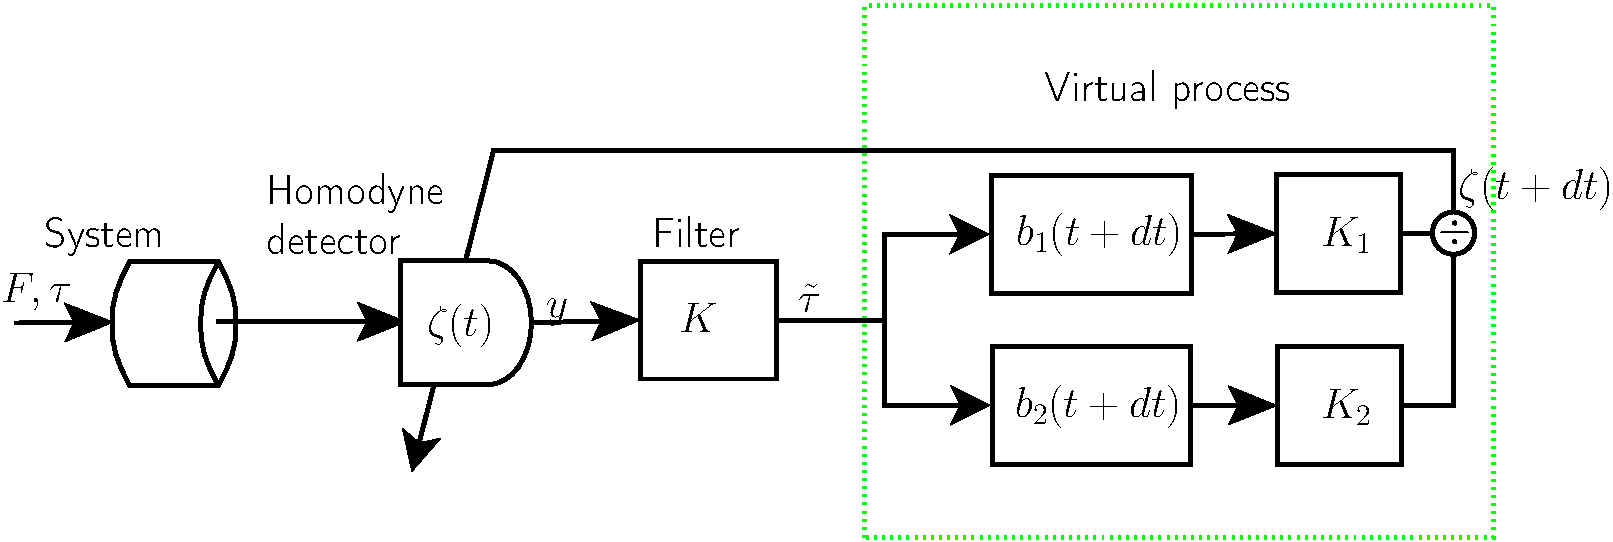
\includegraphics[width=0.95\textwidth]{process}}
\caption{Adaptive measurement scheme}
\label{pic:adaptive_process}
\end{figure}

The procedure of estimation is similar to described in previous section, but there are some significant differences.
Each time step we make two stage procedure (see Fig.\ref{pic:adaptive_process}):

\begin{enumerate}
 \item Estimation of arrival time.
  
On this stage we use all previous collected data for estimation the arrival time. At time $t$ we get some output from homodyne detector $y(t)$. Then we can use filter to get some estimation of arrival time $\tilde{\tau}$. This procedure is in some sense classical, because we use here only data that we have already collected for estimation the arrival time (the strict mathematical description we will provide below)
 \item Choice of optimal homodyne angle

In order to understand this stage we should turn to so-called variational measurements \cite{Vyatchanin1998m}. It uses correlation between measurement noise and back-action noise to evade the back-action. It can be shown mathematically (see Appendix \ref{appx:variational}) that in this case there's filtering function that lets us avoid the back-action.
The only restriction of this procedure is that we have to know arrival time. The same idea lyes in our procedure.

We use estimated arrival time to proceed back-action evading measurements. First we predict two quadratures $\hat{b}_{1,2}$ for next two time steps. We have to use two-steps because back-action affects on the system with time delay, so we can choose the optimal homodyne angle $\zeta(t+dt)$ for evading the back-action at time $t+2dt$. 
This procedure: prediction of quadratures, filtering and calculating the homodyne angle for the next step we do ``in our minds'' and we assume that it takes no time to do this, so it's like some virtual process (see Fig. \ref{pic:adaptive_virtual} )
\end{enumerate}
\begin{figure}
 \center{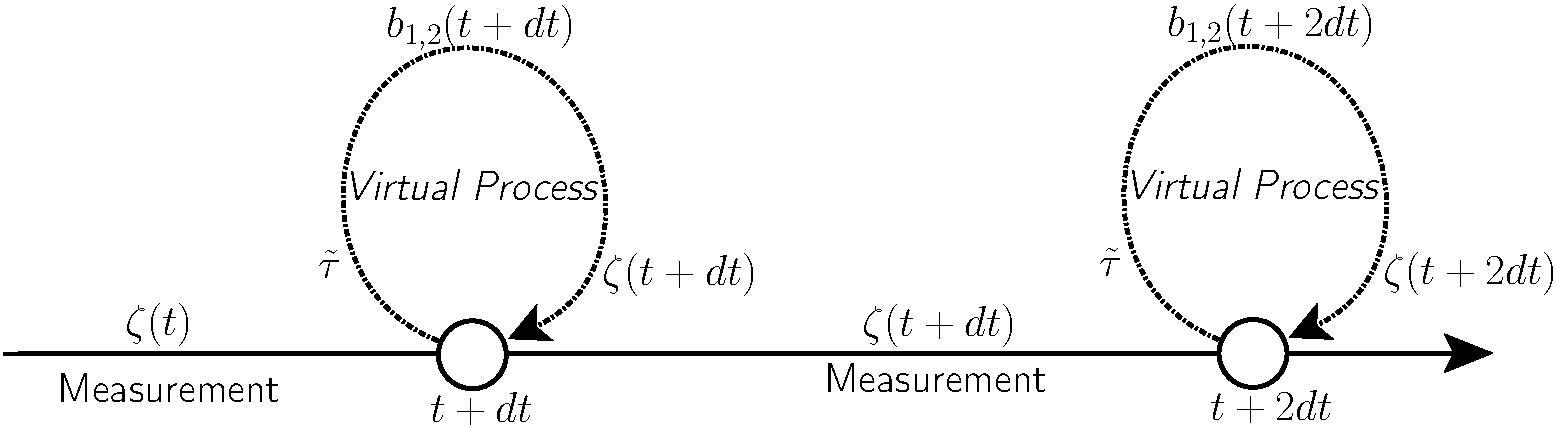
\includegraphics[width=0.9\textwidth]{process_sceme}}
\caption{Scheme for understanding the second stage.}
\label{pic:adaptive_virtual}
\end{figure}

This procedure can be described with a strict mathematics.
\subsubsection{First stage}
In our case we can write output as
\begin{equation}
 y(t)=\mathbb{C}(t)x+n(t)
\end{equation}
Here:
\begin{align}
& \mathbb{C}(t) = \sin\zeta(t)
\begin{bmatrix}
 \sin\omega_mt, & -\cos\omega_mt
\end{bmatrix}
\\
&
x=
\begin{bmatrix}
 A_c\\
A_s
\end{bmatrix}
\\
& n(t) = 
\begin{bmatrix}
 \cos\zeta(t), & \sin\zeta(t)
\end{bmatrix}
\begin{bmatrix}
 n_1(t)\\
n_2(t)
\end{bmatrix}
% =\mathbb{F}(t)\mathbb{N}(t)
\end{align}

We want to estimate two parameters $A_{c,s}$, using the filtering approach, as we mentioned before. In Appendix \ref{filtering} we show, how to get filtering function and derive estimation (see Eq.\ref{appx:est}):
\begin{equation}
 \tilde{x} =
\begin{bmatrix}
 \tilde{A_c}\\
\tilde{A_s}
\end{bmatrix}
= (\mathbb{D}^T\mathbb{N}^{-1}\mathbb{D})^{-1}\mathbb{D}^T\mathbb{N}^{-1}\mathbf{y}
\end{equation}

Here measurement matrix is
\begin{equation}
 \mathbb{D} = 
\begin{bmatrix}
 \mathbb{C}(t_0) \\
 \mathbb{C}(t_1) \\
 \vdots\\
 \mathbb{C}(t)
\end{bmatrix},
\end{equation}
signal vector is
\begin{equation}
 \mathbf{y} = 
\begin{bmatrix}
 y(t_0)\\
 y(t_1)\\
\vdots\\
y(t)
\end{bmatrix}
\end{equation}
and noise matrix is
\begin{equation}
 \mathbb{N} = 
\begin{bmatrix}
 \mean{n(t_0),n(t_0)} & \mean{n(t_0),n(t_1)} & \hdots & \mean{n(t_0),n(t)} \\
\mean{n(t_1),n(t_0)} & \mean{n(t_1),n(t_1)} & \hdots & \mean{n(t_1),n(t)} \\
\vdots & \vdots & \ddots & \vdots \\
\mean{n(t),n(t)} & \mean{n(t_1),n(t)} & \hdots & \mean{n(t),n(t)} \\
\end{bmatrix}
\end{equation}
where
\begin{equation}
 \mean{n(t_i)n(t_j)} = 
\begin{bmatrix}
 \cos\zeta(t), & \sin\zeta(t)
\end{bmatrix}
\begin{bmatrix}
 \mean{n_1(t_i),n_1(t_j)} & \mean{n_1(t_i),n_2(t_j)}\\
 \mean{n_2(t_i),n_1(t_j)} & \mean{n_2(t_i),n_2(t_j)}
\end{bmatrix}
\begin{bmatrix}
 \cos\zeta(t_j)\\ \sin\zeta(t_j)
\end{bmatrix}
\end{equation}

and

\begin{equation}\label{noises}
 \begin{cases}
  \means{\hat{n}_1(t)\hat{n}_1(t')}=&\frac{1}{2}\delta(t-t'),\\
  \means{\hat{n}_1(t)\hat{n}_2(t')}=&\frac{\alpha^2}{2\hbar}G(t'-t)\Theta(t'-t),\\
  \means{\hat{n}_2(t)\hat{n}_1(t')}=&\frac{\alpha^2}{2\hbar}G(t-t')\Theta(t-t'),\\
  \means{\hat{n}_2(t)\hat{n}_2(t')}=&\frac{1}{2}\delta(t-t')+\frac{\alpha^4}{4\hbar^2 m^2 \omega_m^2}\bigl(t'\cos\omega_m(t-t')-\frac{1}{\omega_m}\cos\omega_mt\sin\omega_mt'\bigr)\Theta(t-t')+\\
&+\frac{\alpha^4}{4\hbar^2 m^2 \omega_m^2}\bigl(t\cos\omega_m(t-t')-\frac{1}{\omega_m}\cos\omega_mt'\sin\omega_mt\bigr)\Theta(t'-t)+\\&+ \frac{\alpha^2}{2 m w \hbar}\cos\omega_m(t-t').
 \end{cases}
\end{equation}
% \begin{align}
% \bf{V}_1 =& 
%   \begin{bmatrix}
%   \begin{tabular}{cc|cccc}
%    $\mean{A_c, A_c}$ & $\mean{A_c, A_s}$&$\mean{A_c,y(t_1)}$ & $\mean{A_c,y(t_2)}$ & \ldots & $\mean{A_c,y(t)}$\\
%   $\mean{A_s, A_c}$ & $\mean{A_s, A_s}$&$\mean{A_s,y(t_1)}$ & $\mean{A_s,y(t_2)}$ & \ldots & $\mean{A_s,y(t)}$\\
%    \hline
%    $\mean{A_c, y(t_1)}$ & $\mean{A_s, y(t_1)}$ & $\mean{y(t_1),y(t_1)}$ & $\mean{y(t_1),y(t_2)}$ & \ldots & $\mean{y(t_1),y(t)}$\\ 
%   $\mean{A_c, y(t_2)}$ & $\mean{A_s, y(t_2)}$ & $\mean{y(t_2),y(t_1)}$ & $\mean{y(t_2),y(t_2)}$ & \ldots & $\mean{y(t_2),y(t)}$\\
%   $\vdots$ & $\vdots$ & $\vdots$ & $\vdots$ & $\ddots$ & $\vdots$\\
%  $\mean{A_c, y(t)}$ & $\mean{A_s, y(t)}$ & $\mean{y(t),y(t_1)}$ & $\mean{y(t),y(t_2)}$ & \ldots & $\mean{y(t),y(t)}$\\ 
% %   $\mean{x_0, b1(0)}$ & $\mean{b_1(0),b_1(0)}$ & $\mean{b_1(0),b_2(0)}$ & \ldots & $\mean{b_1(t+dt),b_1(t+dt)}$ & $\mean{b_1(t+dt),b_2(t+dt)}$\\ 
% % $\mean{x_0, b2(0)}$ & $\mean{b_2(0),b_1(0)}$ & $\mean{b_2(0),b_2(0)}$ & \ldots & $\mean{b_2(t+dt),b_1(t+dt)}$ & $\mean{b_2(t+dt),b_2(t+dt)}$\\ 
% %  
%   \end{tabular}
%  \end{bmatrix}
% =\\=&
% \begin{bmatrix}
%   \begin{tabular}{c|c}
%   $V_{xx}^{(1)}$ & $V_{xy}^{(1)}$\\
%   \hline
%   ${V_{xy}^{(1)}}^T$ & $V_{yy}^{(1)}$
%  \end{tabular}
%  \end{bmatrix}
% \end{align}

% Then we calculate estimation for vector 
% \begin{equation}
%   \tilde{\mathbb{X}} = 
%  \begin{bmatrix}
%   \tilde{A}_c \\ \tilde{A}_s
%  \end{bmatrix}
% = V_{xy}^{(1)}{V_{yy}^{(1)}}^{-1}y
% \end{equation}
Using this estimation,we get the estimated arrival time:
\begin{equation}
 \tilde{\tau} = \frac{1}{\omega_m}\arctan \frac{\tilde{A}_s}{\tilde{A}_c}
\end{equation}
This equation describes the estimation for arrival time that we get on each time step.

\subsubsection{Second stage}
In previous step we used the knowledge about measurement results in the past. Now we want to make prediction about next measurement in order to find optimal homodyne angle.
Suppose, that we can make prediction about both quadratures $b_{1,2}$. Then:
\begin{equation}
 \begin{cases}\label{b1b2}
  \hat{b}_1(t) = \hat{a}_1(t) \\
  \hat{b}_2(t) = \hat{a}_2(t)+ I(t) + \frac{\alpha^2}{\hbar}\int\limits_0^{\infty} dt' \, G(t-t') \,\Theta(t-t') \hat{a}(t') + \frac{\alpha}{\hbar}x_0 \sin \omega_m (t-\tilde{\tau})
 \end{cases}
\end{equation}
In back-action term we can use sum instead of the integral. So we can write this integral as product of two vectors:
\begin{equation}
 \I{0}{t}d\tau\, G(t-\tau)a_1(\tau) = \lim\limits_{dt\rightarrow0}\sum\limits_{i=1}^NG(t-t_i) a_1(t_i) dt = \lim\limits_{dt\rightarrow0} 
\begin{bmatrix}
 G(t-t_1), & G(t-t_2), & \hdots, & G(t-t_N)
\end{bmatrix}
\begin{bmatrix}
 a_1(t_1)\\a_1(t_2)\\\vdots\\a_2(t_N)
\end{bmatrix}
dt
\end{equation}
where $t_i = i\,dt, t_N = t$
For any moment of time $t$ we can compute back-action matrix as:
\begin{equation}
 \begin{bmatrix}
  BA(t_1)\\BA(t_2)\\\vdots\\BA(t)
 \end{bmatrix}
=\alpha
\begin{bmatrix}
 0 & 0 & 0 &\hdots & 0\\
 G(t_2-t_1) &0 &0 &\hdots & 0\\
 G(t_3-t_1) &G(t_3-t_2) &0 &\hdots & 0\\
\vdots &\vdots &\vdots &\ddots & \vdots\\
G(t-t_1) &G(t-t_2) &G(t-t_3) &\hdots & 0
\end{bmatrix}
\begin{bmatrix}
 a_1(t_1)\\a_1(t_2)\\\vdots\\a_2(t)
\end{bmatrix}
dt
\end{equation}

Here we can use the same filtering approach, but now for two quadratures:
\begin{equation}
 \begin{bmatrix}
  \hat{b}_1(t+dt)\\ \hat{b}_2(t+dt)
 \end{bmatrix}
=
\begin{bmatrix}
 0 \\ \frac{\alpha}{\hbar} \sin \omega_m(t+dt)
\end{bmatrix}
x_0 + I(t)+
\begin{bmatrix}
 \hat{n}_1(t+dt) \\ \hat{n}_2(t+dt)
\end{bmatrix}
\end{equation}

Then covariation matrix between signal and output would be:
{\tiny
\begin{equation}
\hspace{-2cm} \bf{V}_2 = 
 \begin{bmatrix}
 \begin{tabular}{c|c|cccc}
   $\mean{x_0, x_0}$ & $V_{xy}^{(1)}$ & $\mean{x_0,b_1(t+dt)}$ & $\mean{x_0,b_2(t+dt)}$ & $\mean{x_0,b_1(t+2dt)}$ & $\mean{x_0,b_2(t+2dt)}$\\
   \hline
   ${V_{xy}^{(1)}}^T$  & $V_{yy}^{(1)}$ & 
$\begin{matrix}
\mean{y(t_1),b_1(t+dt)}\\
\vdots \\
\mean{y(t),b_1(t+dt)} \\
\end{matrix}$ & $\begin{matrix}
\mean{y(t_1),b_2(t+dt)}\\
\vdots\\
\mean{y(t),b_2(t+dt)}\\
\end{matrix}$ &
$\begin{matrix}
\mean{y(t_1),b_1(t+2dt)}\\
\vdots \\
\mean{y(t),b_1(t+2dt)} \\
\end{matrix}$ & $\begin{matrix}
\mean{y(t_1),b_2(t+2dt)}\\
\vdots\\
\mean{y(t),b_2(t+2dt)}\\
\end{matrix}$\\
\hline
$\mean{b_1(t+dt),x_0}$ & 
$\begin{matrix}
\mean{b_1(t+dt),y(t_1)} & \ldots & \mean{b_1(t+dt),y(t)} \\
\end{matrix}$ & $\mean{b_1(t+dt),b_1(t+dt)}$ & $\mean{b_1(t+dt),b_2(t+dt)}$ & $\mean{b_1(t+dt),b_1(t+2dt)}$ & $\mean{b_1(t+dt),b_2(t+2dt)}$\\
$\mean{b_2(t+dt),x_0}$ & 
$\begin{matrix}
\mean{b_2(t+dt),y(t_1)} & \ldots & \mean{b_2(t+dt),y(t)} \\
\end{matrix}$ & $\mean{b_2(t+dt),b_1(t+dt)}$ & $\mean{b_2(t+dt),b_2(t+dt)}$& $\mean{b_2(t+dt),b_1(t+2dt)}$ & $\mean{b_2(t+dt),b_2(t+2dt)}$\\
$\mean{b_1(t+2dt),x_0}$ & 
$\begin{matrix}
\mean{b_1(t+2dt),y(t_1)} & \ldots & \mean{b_1(t+2dt),y(t)} \\
\end{matrix}$ & $\mean{b_1(t+2dt),b_1(t+dt)}$ & $\mean{b_1(t+2dt),b_2(t+dt)}$ & $\mean{b_1(t+2dt),b_1(t+2dt)}$ & $\mean{b_1(t+2dt),b_2(t+2dt)}$\\
$\mean{b_2(t+2dt),x_0}$ & 
$\begin{matrix}
\mean{b_2(t+2dt),y(t_1)} & \ldots & \mean{b_2(t+2dt),y(t)} \\
\end{matrix}$ & $\mean{b_2(t+2dt),b_1(t+dt)}$ & $\mean{b_2(t+2dt),b_2(t+dt)}$ & $\mean{b_2(t+2dt),b_1(t+2dt)}$ & $\mean{b_2(t+2dt),b_2(t+2dt)}$
  \end{tabular}
 \end{bmatrix}
\end{equation}
}
Then filter is
\begin{equation}
\mathbb{K}_2 = V_{xy}^{(2)}{V_{yy}^{(2)}}^{-1} = 
\begin{bmatrix}
 K_{y(t_1)}\\K_{y(t_2)}\\\vdots\\K_{y(t)} \\K_1(t+dt)\\K_2(t+dt)\\K_1(t+2dt)\\K_2(t+2dt)
\end{bmatrix}
\end{equation}
where 
\begin{equation}
  V_{xy}^{(2)} = 
\begin{bmatrix}
 V_{xy}^{(1)}, & \mean{x_0,b_1(t+dt)}, & \mean{x_0,b_2(t+dt)} & \mean{x_0,b_1(t+2dt)}, & \mean{x_0,b_2(t+2dt)}
\end{bmatrix}
\end{equation}
Here we remember that we have to get homodyne angle at time $t+dt$ to evade the back-action at time $t+2dt$
Then due to the fact that readout is $$Y(t+dt)=K_1(t+dt) b_1(t+dt) + K_2(t+dt) b_2(t+dt) = g \cos\zeta(t+dt)b_1(t+dt)+g\sin\zeta(t+dt)b_2(t+dt)$$ 
we can find homodyne angle as
\begin{equation}
 \zeta(t+dt) = \arctan\frac{K_2(t+dt)}{K_1(t+dt)}
\end{equation}

If we compute all the covariation functions, we get:
\begin{equation}
 \means{x_0,x_0} = \sigma_{x_0}
\end{equation}
\begin{align}
& \means{x_0,b_1(t+dt)} = 0\\
& \means{x_0,b_2(t+dt)} = \frac{\alpha}{\hbar}\sigma_{x_0} \sin\omega_m(t+dt-\tilde{\tau})
\end{align}

And output correlations with signal at time $t_j<t_i$:
\begin{equation}
\begin{cases}
\means{b_1(t_i),y(t_j)} = 0\\
\means{b_2(t_i), y(t_j)} = \means{b_2(t_i),b_1(t_j)}\cos\zeta(t_j) + \means{b_2(t_i),b_2(t_j)}\sin\zeta(t_j)
\end{cases}
\end{equation}